

\documentclass[11pt,a4paper,titlepage,oneside]{article}

\usepackage[most]{tcolorbox}
\usepackage{geometry}
\usepackage{svg}

\usepackage{hyperref} %links
\usepackage{xurl}

\usepackage[document]{ragged2e} %floating text
\usepackage{helvet} %font
\usepackage{tocloft} % dots in table of contents sections

\usepackage{lipsum, multicol}
\usepackage{fancyhdr}
\usepackage{listings}


% citaitons
\usepackage{natbib}

% hypthenationrules
\usepackage[T1]{fontenc}



%redefine the entire fucking bib environment so we dont have the horisontal spacing
% this was generated entirely by chatgpt

\makeatletter
\renewenvironment{thebibliography}[1]
  {\section{Lähteet}%
   \@mkboth{\MakeUppercase{\refname}}{\MakeUppercase{\refname}}%
   \list{\@biblabel{\@arabic\c@enumiv}}%
        {\settowidth\labelwidth{\@biblabel{#1}}%
         \leftmargin\labelwidth
         \advance\leftmargin\labelsep
         \setlength\itemindent{-\labelwidth}
         \setlength\itemsep{10pt} % Change this value to adjust the space between items
         \@openbib@code
         \usecounter{enumiv}%
         \let\p@enumiv\@empty
         \renewcommand\theenumiv{\@arabic\c@enumiv}}%
   \sloppy
   \clubpenalty4000
   \@clubpenalty \clubpenalty
   \widowpenalty4000%
   \sfcode`\.\@m}
  {\def\@noitemerr
    {\@latex@warning{Empty `thebibliography' environment}}%
   \endlist}
\makeatother





%this is such a shitshow lmao

\hypersetup{
    colorlinks=false,
    citecolor=black,
    filecolor=black,
    linkcolor=black,
    linkbordercolor=1 1 1,
    citebordercolor=1 1 1,
    pdfborderstyle={/S/U/W 1},
    urlbordercolor=0 0 1,
    urlcolor=blue
}
\urlstyle{same}



\geometry{
    a4paper,
    left=3cm,
    right=2.5cm,
    top=3cm,
    bottom=2.5cm
}

%remove random margin on side ? idk what happend
%\setlength{\oddsidemargin}{0pt}



%custom reusable colorbox rules
\newtcolorbox{simplebox}{colback=white, sharp corners, boxrule=1pt }


\renewcommand{\contentsname}{Sisällys} % override Contents => Sisallys on table of contents

\renewcommand{\familydefault}{\sfdefault} % set font

\renewcommand{\cftsecleader}{\cftdotfill{\cftdotsep}} % dots for sections

\renewcommand{\bibsection}{\section{Lähteet}}

\setlength{\headheight}{13.6pt}


\def\filename{src/oppari.tex}



\def\testmode{1}






\newcommand\wordcount{
    \immediate\write18{texcount -sub=section \filename{} -inc  | grep Section | sed -e 's/+.*//' | sed -n \thesection p > 'count.txt'}
(\input{count.txt}words)}


\newcommand{\inputf}[1]{\def\filename{#1}\input{#1}}


\newcommand\filewcount{
    \immediate\write18{texcount -1 -sum \filename{} > count.txt }
    \input{count.txt} words }


% jos on testi definetty niin tee 
\newcommand{\istest}[2]{\ifx\testmode\undefined #2 \else #1 \fi}


% testi section näyttää word countin siltä sectionilta jos ei testi niin sitten näytä vain normaali section
\newcommand{\tsection}[2]{\istest{#1{#2\\} \wordcount \\ \medskip }{#1*{#2}}}


\newcommand{\pagesection}[1]{\istest{\section{#1}  }{\section*{#1}}}
\newcommand{\pagesubsection}[1]{\istest{\subsection{#1}  }{\subsection*{#1}}}


% adds page with everything
\newcommand{\addPage}[2]{
    \def\filename{#1}
    \pagesection{#2}
    \istest{ \filewcount \medskip }{}
    \input{#1}
}



% OPPARI SPESIFIC

\newcommand{\addPageOp}[2]{
    \def\filename{#1}
    \pagesubsection{#2}
    \istest{ \filewcount \medskip }{}
    \input{#1}
}

%lab citation style
\newcommand{\labcite}[1]{\setcitestyle{aysep={},open={(},close={.)}}\citep{#1}{}}

%lab citation style
\newcommand{\labciteend}[1]{\setcitestyle{aysep={},open={(},close={).}}\citep{#1}{}}

\newcommand{\labimgcite}[1]{\setcitestyle{aysep={},open={(},close={)}}\citep{#1}{}}

\newcommand{\hurl}[1]{\href{#1}{{\underline{\textcolor{blue}{#1}}}}}


% counter kuville
\newcounter{imgCounter}
\setcounter{imgCounter}{0}

\newcommand{\getImgCount}{
\addtocounter{imgCounter}{1}
\theimgCounter
}


% counter kaavioille
\newcounter{chartCounter}
\setcounter{chartCounter}{0}

\newcommand{\getChartCount}{
\addtocounter{chartCounter}{1}
\thechartCounter
}



\usepackage[finnish]{babel}
















% ------------------------------ BEGIN DOCUMENT ------------------------------ %
\begin{document}

\pagestyle{empty}


%------------------------------ COVER PAGE ------------------------------ %


\includegraphics[width=5cm,height=1cm]{./src/labimg.jpg}

\vspace{86mm}
\huge
\textbf{Kehityksen seuranta}
\newline

\large

\vspace{5mm}
\textbf{Oppimispäiväkirja}
\normalsize

\vspace{90mm}

LAB-ammattikorkeakoulu \newline
\vspace{2mm}
Tieto-ja tietolikenadsfklj, Insinööri (AMK) \newline
\vspace{2mm}
2024 \newline
\vspace{2mm}
Kimi Malkamäki

\newpage




%------------------------------ FIRST PAGE OF ABSTRACT ------------------------------ %
\begin{tabular}{ | l | }

    %hack for the tiivistelmä line
    \multicolumn{1}{l}{
        \begin{minipage}{6cm}
            \hspace{1mm}
            
        \end{minipage}
        \begin{minipage}{4.25cm}
            \hspace{1mm}
        \end{minipage}
        \begin{minipage}[t][1.95cm][t]{3.62cm}
            \large
            \textbf{ Tiivistelmä }
        \end{minipage}
    }\\

    \hline
    \begin{minipage}[b]{6cm}
        tekijä(t)
        \newline
        kimi malkamäki 
    \end{minipage}%
    % 2x2
    \begin{minipage}{8.5cm}
        \begin{tabular}{ | l | c | }
            \begin{minipage}[t][1cm][t]{4.25cm}
                julkaisun laji
                \newline
                Opinnäytetyö, AMK
            \end{minipage} & %
            %
            \begin{minipage}{3.62cm}
                valmistusaika
                \newline
                2024
            \end{minipage} \\ \hline%
            %
            \begin{minipage}[t][1cm][t]{4.25cm}
                sivumäärä
                \newline 
                xx+xx
            \end{minipage}
            &  \\ \hline
        \end{tabular}
    \end{minipage}%
    % end of 2x2
      \\ \hline

    \begin{minipage}[t][2cm][t]{8cm}
    Työn nimi 
        \newline 
    ammatissa kasvaminen 
        \newline 
    oppimispäiväkirja  
    \end{minipage}\\ \hline

    \begin{minipage}[t][1.5cm][t]{10cm}
    tutkinto ja koulutusala.\newline  tietoviestintätekniikka insinööri amk  

    \end{minipage}\\ \hline

    \begin{minipage}[t][7cm][t]{5cm}
    tiivistelmä: \newline lorem ipsim
    \end{minipage}\\ \hline

    \begin{minipage}[t][2cm][t]{5cm}
    avain sanat
    \end{minipage}\\ \hline

\end{tabular}

\newpage



% ------------------------------ SECOND PAGE OF ABSTRACT ------------------------------ %

tiivistelmä








\newpage


% ------------------------------ TABLE OF CONTENTS ------------------------------ %

%keep page numbers off
\setcounter{page}{0}
\pagestyle{empty}
\pagenumbering{gobble}

\tableofcontents





\newpage



% ------------------------------- TERMISTÖ ------------------------------- %


TERMISTÖ
\bigskip

(tiedän ettei termistö kirjoiteta tällä formaatilla. tämäkin on hyvin kesken)
\bigskip
 
%this needs to be aligned cannot be like this make minipage maybe
ECMAscript = skriptaus-kieli standardi 
\bigskip

DOM = Document Object Model 
\bigskip

puu = datastruktuuri(selitä paremmin)
\bigskip

VDOM = virtual DOM
\bigskip

Transpilaatio = ohjelmointi keilen kääntäminen toiseen ohjelmointikieleen
\bigskip

CSS = Cascading Style Sheets
\bigskip



\newpage





% ------------------------------- CONTENT PRELUDE COMMANDS ------------------------------- %
%enable page counting
\pagenumbering{arabic}
\clearpage
\setcounter{page}{1}

%set heaader and footer
\pagestyle{fancy}
%%
\lfoot{}
\cfoot{}
\rfoot{}
%%
\lhead{}
\chead{}
\rhead{\thepage}
%%
\renewcommand{\headrulewidth}{0pt}
\renewcommand{\footrulewidth}{0pt}
%\newcommand{\n}{\newline\vspace{20mm}}











\section{Johdanto}              % ------------------------------- JOHDANTO ------------------------------- %



% jos tulee niin sitten jotain siitä että web suunnittelu liikkuu nopeaseti ja siellä on kokoajan uusia teknologioita
%mutta pohjalta ne perustuu samoihin periaatteisiin.

% tullaanko tekemään seuranta vai jos tulee tarpeeksi tekstiä niin onko ok vaan tehdä normi oppari tästä
% jos tavoitteena olisis se uuden featuren lisääminen





%structures

% it lorem ipsum

% opparin tavoite
% kunnon maininta päiväkirja mallista sillä tässä mainitaan seurantajakso
% ennen kun sanotaan seurantajakso pitää vissiin mainita mitä seurataan ja miksi

% starttaamon intro






% jotain siitä että teknologiat tulee ja menee  ja startupit yrittää päästä mukaan koska siinä on paljon rahaa liikenteessä
(lorem tekstiä menee uusiks)\\ %tää pitäis kijoittaa uudellee ihan kokonaan mutta jotain samantyylistä tekstiä
teknologia ala on nopeasti liikkuva. 
Monet uudet teknologiat ilmestyvät ja vanhentuvat hyvin nopeasti
Suositun tuotteen tai teknologian kehittäminen ja onnistuneesti markkinoille saanti on hyvin tuottava liikemalli, 
mutta monet ketkä yrittää epäonnistuvat.\citemissing
Tämä tuo haasteita alalla työskenteleville ammattilaisille, 
sillä ammatitlaisen pitää olla kokoajan ajantasalla uusista teknologioista ja työntavoista, että voi pysyä alan mukana.

%something more ab this
\medskip


% ei mainita liitettä tässä. sanotaan vaan että on päiväkirja mainen ja että on seurantajakso 
%eli kokonaan alusta ja uusiks
Opinnäitetyö on kirjoitettu päiväkirja mallisesti
ja ennen opinnäytettyön kirjoittamista suoritettiin 13 viikon seurantajakso, jossa
% mitä tehtiin uusiks
kirjattiin ja (jotain) mitä tehtiin ja mitä opittiin viikoittan.
% selitys siitä miksi tämä on hyvä ja miten se liittyy ylempääänn kappaleeseen
Tämä antaa hyvän silmäyksen työskentelemisestä ohjelmistokehittäjänä ja haasteista mitkä ilmeentyvät päivittäin
% jotain lisää siitä että pvkirja antaa silmäyksen elämään itse ammattilaisena,
% jolla on juuri ongelmia mitkä kuvattiin  ekassa kappaleessa
%tässä voi olla joku concrete esimerkki siitä mitä tehtiin ja mitä tehdään
Seurantajakson aikana opin...% jotain itse casesta 
%more text
\medskip

%tässä opparisas ei oikein seurata vaan kirjoitetaan vaan jutuista mitä tehtiin emt

% tätä ennen tulee jotain tekstiä itse tavoite sanotaan tiivistelmässä vissiinkin
Opinnäytettyön tavoitteena on seurata kehitymistä ja teknologoiden oppimista 13 Viikon seurantajakson aikana.

%more text
\medskip


%Opinnäitetyö on kirjoitettu päiväkirja mallisesti.
% ja ennen opinnäytettyön kirjoittamista suoritettiin 13 viikon seurantajakso, jossa
% kirjattiin ja (jotain) mitä tehtiin ja mitä opittiin viikoittan.

%Opinnäitetyö on kirjoitettu päiväkirja mallilla,



%selitys starttaamosta ja mistä se tekee/haluaa

Opinnäytetyö toteutettiin Starttaamo Oy:ssä. Starttaamo on suomalainen startup yritys, joka pyrkii ratkomaan ongelmia työergonomian kanssa.
Startupin pää tavoitteena on vähentää sairaslomia saamalla työntekijät noudattamaan, alojen ammattilaisten suunnittelemien liikunta- ja ruokavalio-ohjelmia. 
% scuffed af.. web alusta jota kehitin...  jotenkin paremmin se että olin kehittämässä sitä mukana.
Yrityksen pää myyntituote on web-alusta, jonka kehityksen mukana olin.
%
Alustan kehittämisessä sain mahdollisuuden työskennellä tuotantoympäristössä ja ....
Olin mukana suunnittelussa ja ominaisuuksien ohjelmoinnissa. sain myös kokemusta ilmeentyvien ongelmien korjaamisesta.

%more
\medskip










\newpage
\section{Lähtötilanne}         % ------------------------------- LÄHTÖTILANNE ------------------------------- %



% nykyisen työtehtävän analyysi
% eli mainitaan jotain työtehtävästä ja mitä siellä on
% voi mainita käytetyistä teknologoiista

% kehittämis tarve
% ei oikeaa kokemusta
% heikko web kehitys kookemus
% oikean alustan kanssa kokemusta on vähän



%ehkä rewrite kokonaan
%struktuurilla

%mikä on tietotaito ennen alkamista

% mitä kehitystarpeita
% analyysi nopeasti jutuista minkä kanssa tulen tekemään ja mitä haluan oppia

% mitä mikä oli alustan tilanne ennen alkamista ja mitä minulle annettiin tehtäväksi
% osallistua alustan kehittämiseen ja kehitykseen
% palavereissa oleminen tekeleiden näyttäminen/esittely jne

%fix this shit
Ennen opinnäytetyön kirjoittamista ja seurantajakson alkamista olin opiskellut LAB ammattikorkeakoulussa XX lukukautta ja
olin opinnäytetyön kirjoituksen aikana neljännen vuoden tieto- ja viestintätekniikkan opiskelia.
Vaikka minulla ei ollut aijempaa aijempaa työkokemusta tieto- ja viestintätekniikkan alalta ennen harjoituksen alkamista,
olin koulutuksen aikana saanut laajan pohjan ohjelmoinnista,
sen perusteista ja muista tieto- ja viestintätekniikan alan taidoista esim. versionhallinnasta, tietokannoista sekä web suunnittelusta.
Teoriapohja ei kuitenkaan aina riitä työelämässä, joten uusiin olosuhteisiin soveltuminen ja uusien asioiden oppiminen on oleellista.
\medskip



% kehityksen tarve. 
Harjoituksen aikana halusin oppia web alustojen kanssa työskentelystä ja projektissa käytetyistä teknologioista.
% ehkä voi lisätä, koska sitä minulla ei ollut. tai jotain muuta vastaavaa
%
Halusin myös kokemusta työskennellä isommassa koodipohjassa, jota muutkin henkilöt ovat olleet suunnittelemassa.
Isommat projektit vaativat palavereita ja yhteenvetoja, että kaikki työntekijät pysyvät ajantasalla.
Sosiaaliset taidot ja kyky selittää teknisiä asioita asiakielellä on myös taito, 
jota en ollut ennen harjoittelua tarvinnut, mutta huomasin sen olevan oleellinen osa työelämää.
Viikottaisten palavereisiin osallistuminen ja viikon aikana tehtyjen töiden esittely ja selittäminen on oleellinen osa isommassa projektissa työskentelemistä.
\medskip


% jotain lisää web alustan kanssa tekemisistä
%en tiedä miten tän lausuu siten että se sopii lähtötilanteeseen
% miten tää kiroitetaan siten että se on työtehtävän analyysiä

Web sovelluksen kehittämisessä tulee esiin haasteita, joita ei tule muussa sovelluskehityksessä.
Sovellukset koostuvat useimmiten monesta osasta, kuten frontend backend ja tietokanta.
Nämä osat pitää olla kokoajan yllä ja yhteyksissä toisiinsa sovelluksien toimimiseen ja niiden katkeaminen voi
johtaa sovelluksen toimimattomuuteen.
% 
Myös palvelin- tai muut sovellus virheet voivat kaataa koko sovelluksen kaikille käyttäjille. 
%
Web sovelluksien kehittämisessä on myös etuja tavalliseen sovelluskehitykseen verrattuna, kuten 
web sovelluksen päivityksen saanti käyttäjille on nopeaa ja kaikki käyttäjät saavat päivityksen samanaikaisesti.
\medskip

% alustan tilanne ja työtehtävän analyysi. 
Harjoituksen aika työskentelin Startupin web alustan kanssa. 
Olin mukana sen kehityksessä, suunnittelussa, ominaisuuksien lisäämisessä ja sivustojen ylläpidossa.
Alusta oli käyttöönotettu ennen harjoituksen alkamista ja siellä oli aktiivisia käyttäjiä.
Alusta on ollut käytössä X vuotta ennen harjoituksen alkamista ja sitä ennen X vuotta suunnittelussa.
%
%??
% paljon random shittii on missing sen takii että haluttiin jotakin valmiiksi
Alustan kehityksessä, oltiin tehostettu kehitysnopeuteen,
joten alustalta puuttui monia ominaisuuksia, joita odotetaan web sovelluksesta, 
kuten web sivustojen kääntäminen ja sivustojen toimiminen mobiililaitteilla.
\medskip

























\newpage
\section{Teoria}                % ------------------------------- TEORIA ------------------------------- %



\subsection{Kehitys ympäristö / Teknologia pino}

%yleisesti tässä kappaleessa voisi olla ainakin yksi kokonainen sivullinen tekstiä
%ainakin sen verran pitäisi saada kirjoitettua




% scuffed af kun käytettyjen teknologioiden lukee kahesti päällekkäin

% vähän paremmin selitys markkinoille pääsemisenn
Startup- ja muut kasvuyritykset, jonka pää tuotteena on sovellus tai muu teknologia, hakee nopeaa ja ketterää kehitystä markkinoilla pärjäämiseen.
% kirjoita kehitys nopeus paremmin
Tämä pitää ottaa huomioon käytettyjen teknologioiden valinnassa, sillä eri teknologioilla on eri kehitysnopeus.
Pohjalla käytettyjen teknologioiden vaihtaminen on erittäin työlästä jälkikäteen,
joten päätös käytetyistä teknologioista tulee määräämään yhtiön kehityksen nopeuden.
Hidas sovelluskehitys voi haitata itse yrityksen mahdollisuuksia selvitä markkinoilla.
\medskip




Teknologia pino pohjautuu MeteorJs kehykseen. Se on suunniteltu nopeaan kehittämiseen ja käyttöönottoon.
Meteor helpottaa kommunikointia käyttöliittymän, palvelimen ja tietokannan kanssa, 
mutta silti antaen vapauden valita muut käytettävät teknologiat, eikä lukitse käyttämään valmiiksi valittuja teknologioita.
Meteor ei määritä käytettyä käyttöliittymä kirjastoa mutta se silti tukee monia suosituimpia kehyksiä ja antaa halpon integraation niihin.
Projekttin on valittu ReactJs kirjasto käyttöliittymän toteutukseen.
Reactin komponentti pohjainen rakenne tekee käyttöliittymä koodista helposti uudelleen käytettävän, nopeuttaen käyttöliittymän rakentamista. 
Myös sen sisään rakennettu reaktiivisuus tilallisilla komponenteilla tuo helpon käyttöliittymä päivityksen.
Meteorilla on hyvä integraatio ReactJs:ssän kanssa. 
Tämä on nähtävillä kun Meteor päivittää automaattisesti käyttöliittymää tietokantamuutoksien tapahduttua. 
Projektissa käytössäoleva tietokanta MongoDB on kanssa hyvin integroitu Meteoriin.
MongoDBn skeematon dokumentti rakenne, tuo helpon tavan päivittää skeemmoja tarpeiden tullen.
%jokunen lause lisää mongodbstä ennen kun seuraava kapale
\medskip



MeteorJs MongoDB ja ReactJs on pohjalla olevat teknologiat, jonka päälle projekti on rakennettu.
Yhdessä näitä kolmea teknologiaa käytten voi luoda monenlaisia nopeuta ja skaalautuvia nettisivuja pienistä projekteista suuriin.
Nämä teknologiat ovat myös suunniteltu nopeaan kehittämiseen, joka tekee niistä hyvän valinnan kasvavalle startup yritykselle.
%more
\medskip









%sitatatti order kussee
\newpage
\subsection{Meteor}                % ------------------------------- Meteor ------------------------------- %



\subsubsection{Meteor yleisesti}



% https://guide.meteor.com/collections.html#mongo-collections
% meteor uses mongo. but it is not manditory





Meteor on full-stack JavaScript web-framework ja on itsessään avoimeen lähdekkoodiin perustuva, \labcite{meteor24b}
poislukien meteorin mukaan paketoimaa mongodb tietokantaa, joka toimii Server Side Public Lisenssillä.\labcite{mongodb24i}
Meteor on suunniteltu nopeaan kehittämiseen monelle laitteille ja nopeaan käyttöönottoon ja se keskittyy isomorphiseen koodiin, 
eli koodiin joka on samanlaista palvelimella kuten clientillä.\citemissing
Meteor ei määritä käytettyä front-end teknologiaa vaan sillä on integraatio moneen yleiseen frontend-framework:kiin, kuten Vue, React, Svelte tai Angular.\labcite{meteor24a}
Tämä antaa lisä joustoa Meteorille sillä se antaa mahdollisuuden monelle sovelluskehittäjälle joilla ei ole kokemusta tietystä front-end teknologiasta.



\medskip

% asio ok mut kirjota paremmin ja uusiks varm gpt on ok täs vaihees
%paremmin alku 
Meteor on fullstack, joten kun sen käynnistää se käynnistää samalla palvelimen ja clientin.
Tiedostorakenteessa on erityks kansioita kuten server ja client jota käyttäen Meteor tietää mitä koodia pitää ladata clientille ja mitä palvelimelle.
%more text




\medskip

    
% https://www.meteor.com/
% viitattu 28.5

% tukee sana pitää vaihtaa sillä me käytetään sitä itemeissä
Lisäksi Meteor tukee monta ominaisuutta kuten. \labcite{meteor24a}
\begin{itemize}
    \item Tukee monta Front-end kirjastoa ja frameworkkkia
    \item Tukee Typescriptiä
    \item Sisään rakennettu käyttäjä systeemi
    \item Toimii monella laitteella
    \item Helppo ja nopea käyttöönottaa 
\end{itemize}
\medskip


Meteor paketoi mukaansa käyttäjä paketin jota käyttäen kehitäjä voi nopeasti luoda authentikaatio järjestelmän.
Käyttäjä paketti antaa helpon integraation muiden kirjautumis palvelujen kanssa kuten facebook, github, google ym. \labcite{meteor24c}
Käyttäjä paketti on myös integroitu muihin Meteorin ominaisuuksiin kuten metodeihin.
%maby more txt



\subsubsection{Meteor metodit}

% kirjoita tämä oikeella oppari tyylillä. idk tuntuu vähän väärältä tässä


% kappale rpc. mikä on ja miten eroaa restful

%enemmän yleis selostusta rps ja restful mikä on ero hyvät ja huonot puolet

Meteor käyttää RPC (eng Remote procedure call) rajapintaa \labcite{meteor24a} perinteisen RESTful rajapinnan sijasta. % ne on asynkroonisia callback funktiolla
Tämä antaa mahdollisuuden clientille kutsua funktioita palvelimella Meteorin kautta.
% joku selitys että metodi on rpc
Meteorin RPC rajapinnat ovat Meteor metodit.
%jotain muuta loremia ennen ku mennään metodit käytännössä vaiheeseen
\medskip


Metodit määritetään ja suoritetaan palvelimella kuten kuvassa \nextImageCount.
%selitä isomorpinen paremmin tässä kontekstissa
%koodi on metodi kutsu on samaa clientillä ja palvelimella joten metodeja voi helpommin uudelleen käyttää 
Metodit tekee myös koodista yksinkertaisemman sillä clientin ei tarvitse tehdä GET tai POST requesteja palvelimelle, kun halutaan palvelimen tehdä jotain. 
Ja koska metodi kutsu on myös isomorphinen, metodeja on helppo uudelleen käyttää palvelimella.
% tutki onko tämä oikea selitys
Metodi funktion "this"{} ominaisuus saa kutsujan kontekstin. 
Tässä kontekstissa voi nähdä esimerkiksi onko kutsuja kirjautunut sisään, tai onko kutsujalla oikeat oikeudet kutsua metodia, 
helpottaen turvallisuuden lisäämista rajapintaan.
\bigskip

% jos tarvitaan lisää niin kuva metodista ja sen kutsumisesta
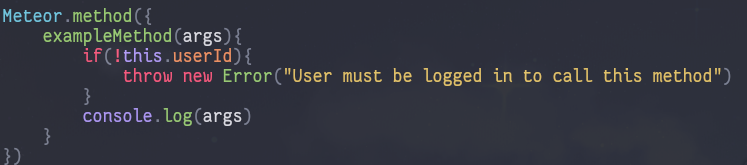
\includegraphics[width=15cm]{src/public/methodexample.png}\\
Kuva \getImgCount {}. Meteor metodin määritelmä
\medskip

% tutki onko tämä accurate selitys asiasta
Kuvassa on meteor metodin määritelmä. "exampleMethod"{} metodi katsoo, onko kutsujalla käyttäjä tunnusta, näin voimme tietää onko kutsuja kirjautunut sisään,
jos käyttäjä ei ole kirjautunut sisään heitämme error viestin, joka välitetään kutsujalle.
Jos käyttäjä on kirjautunut sisään tulostetaan argumentit. 

\medskip




\subsubsection{Meteor ecosysteemi}

% jotain package management
%https://www.linkedin.com/pulse/build-apps-isomorphic-ecosystem-meteorjs-pranav-shah
% 18.6 

%more about athmosphere
%https://guide.meteor.com/using-atmosphere-packages
% 18.6 


% yhdistä lauseet paremmin, elä aloita jokainen lause Meteor sanalla
Meteor ylläpitää omaa paketointi ecosysteemiään.
Meteor paketit ovat isomorphisia, eli ne toimivat palvelimella ja clientillä.\labcite{pranav17}{}
Meteorilla on ensimmäisen osapuolen paketteja, joita itse meteor tiimi ylläpitää ja kolmannen osapuolen paketteja,
% selitä athmosphere paremmin
joita yhteisö ylläpitää. Nämä kolmannen osapuolen paketit voi ladata Meteorin paketti palvelimelle Athmosphere:lle.
%more text
\medskip

%https://guide.meteor.com/atmosphere-vs-npm

Athmosphere on Meteorin ylläpitämä paketti palvelin, johon käyttäjät voivat ladata paketteja tai kirjastoja jotka ovat suunnattu toimimaan MeteorJs:ssän kanssa.
NPM paketit (eng Node package manager) ovat suunnattu toimimaan Node ympäristössä, ja vaikka ratkaisuja on käyttää NPM paketteja selaimella, 
Athmosphere paketit voi hyötykäyttää Meteorin build systeemiä, jonka avulla paketin kehittäjä voi määritellä mitkä osat ladataan selain puolelle ja mitkä palvelimelle.\citemissing



% toinen kappale niin sen pitää olla athmospheresta vissiinkin
% mitä lisää athospheresta






\newpage
\addPageOp{./src/op/react.tex}{React}% ------------------------------- REACT ------------------------------- %






\newpage
\addPageOp{./src/op/mongo.tex}{MongoDB}        % ------------------------------- MONGODB ------------------------------- %













\newpage
\subsection{Responsiiviset käyttöliittymät}        % ------------------------------- Responsive ------------------------------- %

% layout => asettelu

\subsubsection{Responsiivisten käyttöliittymien suunnittelun periaatteet}



%https://alistapart.com/article/responsive-web-design/
% viitattu 19.6




% selitä enemmillä sanoilla ja paremmin eri laitteiden käyttö
Tekniikan parantuessa verkkolaitteiden määrä on kasvanut, ja ihmiset käyttävät enemmän ja enemmän eroavia laitteita verkkosivujen selaamiseen.\citemissing
Kehittäjien pitää ottaa huomioon eri erilaitteiden muuttujat kuten, näytönkoot, kuvasuhde, näytön resoluutio ja käytössä oleva HID.\citemissing
Uusien verkkosivujen luominen ei ole käytännöllistä, sillä niiden niitä pitäisi ylläpitää erikseen työpöytäsivuista.
Saman verkkosivun käytön toiminta useammalla eri laitteella vaatii eri lähestymistapaa verkkosuunnitteluun. 
% layout sana vaihtoon
Sivuston layout pitää pystyä muuttumaan sopivaksi laitteelle.
Verkkosivujen suunnittelua tätä lähestymistapaa kutsutaan responsiiviseksi suunnitteluksi. \citemissing
\medskip



Responsiivinen verkkosuunnittelu on lähestymistapa verkkosivustojen rakentamiseen,
jolla varmistetaan niiden optimaalinen ulkoasu ja toimivuus eri laitteilla näytön koosta huolimatta.\citemissing
Responsiiviset verkkosivut mukautuvat käyttölaitteeseen, siten että ne voisi tarjota yhdenmukaisen käyttökokemuksen käyttölaitteesta riippumatta.
\medskip





\subsubsection{CSS Media query}

%https://developer.mozilla.org/en-US/docs/Web/CSS/CSS_media_queries

CSS (eng Cascading Style Sheets) antaa työkaluja millä kehittäjä voi tietää käytetystä laitteesta.
Näitä kutsutaan Media queryiksi.
Mediaqueryt mahdollistaa selain tai käyttölaite arvojen kyselyn ja testailun, ja mahdollistaa ehdollisen CSS tyylien asettelun.

\medskip



% %https://developer.mozilla.org/en-US/docs/Learn/CSS/CSS_layout/Media_queries

%yritä kirjoittaa tää tohon ylempään 
% asiakieli ja uusiks kirjoitus 
CSS Media Query antaa mahdollisuuden CSS-säännöksen asettamiselle vain silloin kun selain- ja laiteympäristö vastaa määritettyjä sääntöjä. 
%tämä ainakin uusiks
Säännökset voivat olla esimerkiksi "jos näytön koko on pienempi kuin X".
%tämä kanssqa jotenkin paremmin
Media Queryt ovat tärkeä osa repsonsiivista suunittelua ja se antaa mahdollisuuden luoda erilaisia layouttteja riippuen käyttölaitteesta,
sen näytön koosta tai kuvasuhteesta.



%esimerkkejä mediaqueryista tai jotain vastaavaa

%jotain vähän lisää mediaqueryistä








\subsubsection{Asettelu vaihtoehdot}
%https://www.theseus.fi/bitstream/handle/10024/94414/Thesis%20Rogatnev%20Nikita.pdf?sequence=1&isAllowed=y
%https://www.theseus.fi/handle/10024/94414
%reading from this idk if we should cite this. it is a real thing so we could. i would want to read from another source
% cite is 20.6


% this is scetch but accurate. also calls it elastic
%https://www.smashingmagazine.com/2009/06/fixed-vs-fluid-vs-elastic-layout-whats-the-right-one-for-you/
%

% medium looks good
%https://bootcamp.uxdesign.cc/fixed-width-responsive-and-adaptive-layout-what-to-chose-a29c4f93537b

%
%https://learn.onemonth.com/responsive-vs-adaptive-vs-fluid-design/

%https://www.acil.in/between-fixed-fluid-adaptive-and-responsive-layout/

%there is some reading on layouts
% all cited 20.6


%mikä on layout ja miten se näyttää itse sivulla.
% on eri layoutteja ja niille sopivia suunnittelu tapoja jne 

%complete rewrite
On eri tapoja suunnitella sivu elementtien asetteluja jne. kolme näistä on fixed, fluid ja adaptiivinen.\citemissing
\medskip



Kiinteä asettelussa elementit pysyvät samana näyttökoosta huolimatta. 
Kiinteässä asettelussa tulee ongelmia jos näytön koko on pienempi kun sivustolle suunniteltu asettelu, 
sillä joitain elementtejä jäisi näytöstä ulkopuolelle tai saatavissa sivu scrollaamisella.\citemissing
\medskip


Nestämmäisessä asettelussa elementtien koot vaihtuu näytön koon mukaan. 
Verrattuna kiinteään asetteluun elementit eivät jää näytöstä ulkopuolelle sillä elementit skaalautuvat näytönkoon mukaan.
%selitä vähän paremmin
Nestemmäisessä asettelussa tulee silti ongelmia sillä jos elementti on liian pieni sille annetulle tekstille.\citemissing
\medskip


Adaptiivisessä asettelussa elementtien koot ja sijainnit muuttuvat riippuen näytönkoosta.\citemissing
% parempi aloitus ei aloiiteta adaptiivisella
Adaptiivisen asettelun ideana on mukauttaa sivuston elementtien asettelu sopivaksi käytetylle laitteelle.
Kuvassa \nextImageCount {} on esimerrki sivuston asettelustosta, kuvassa {\the\numexpr \theimgCounter + 2 } on esimerkki miltä sivusto voisi näyttää jos käytössä olisi adaptiivinen asettelu.
% sopimaan uusiks
Käyttöliittymän elementit ovat siirtyneet vierekkäisestä asettelusta päällekkäiseen sopimaan pienempään näytönkokoon
%more
\medskip

\bigskip
%kuva adaptiivisesta jotain

%kuvat medium artikkelin giffistä
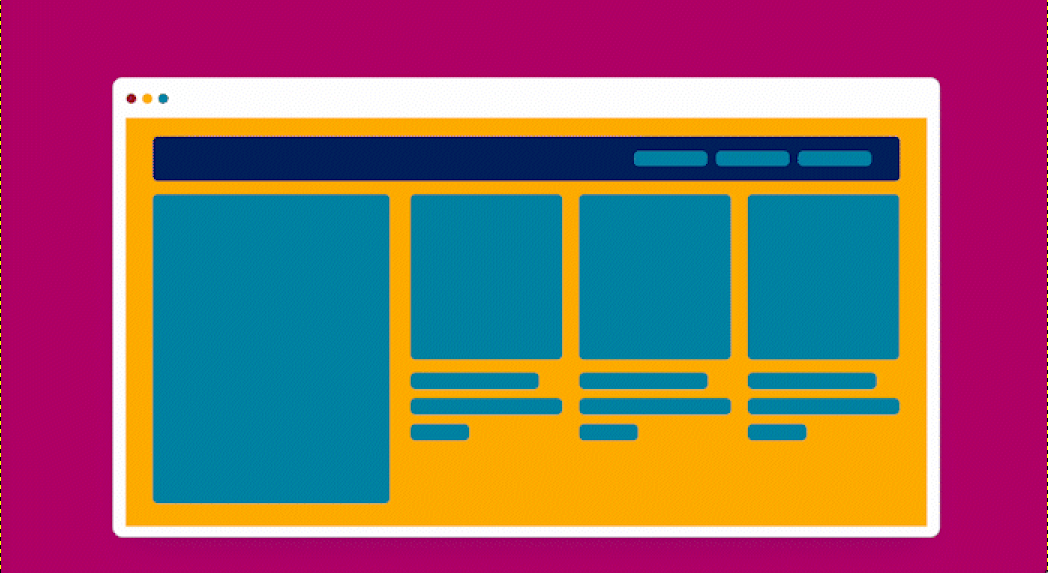
\includegraphics[width = 15cm]{src/public/oppar/adaptiveBig.png}\\
Kuva \getImgCount {}. f adaptiivinen iso\citemissing
 
\bigskip


\includegraphics[width = 15cm]{src/public/oppar/adaptivesmall.png}\\
Kuva \getImgCount {}. f adaptiivinen pieni\citemissing




















\newpage
\subsection{Web sivustojen kääntäminen}

%tämän jos jakaa subsektioneihin niin se veisi enemmän tilaa


% jotain tekstiä siitä miksi kääntää sivustot

% jotain teoriaa käännöksistä yleisesti? what does this mean

% miten käännökset tehdään nettisivuille teknisesti
% jotain vaihtoehtoja ja eri tapoja tehdä käännöksiä


%link tree
% https://www.linkedin.com/pulse/website-translation-how-to-guide-louise-souter





%jotenkin niin vähän tietoa joka ei ole mainos tai jotain liian broad ettei siitä ole hyötyä


\subsubsection{motivaatio verkkosivustojen kääntämiseen}

%miksi kääntää sivustot------------------------------------

% people prefer content in their lenguage
%https://csa-research.com/Featured-Content/For-Global-Enterprises/Global-Growth/CRWB-Series/CRWB-B2C#10Facts
% 11.6


%https://localizejs.com/articles/convince-stakeholders-localization-roi-data
% roi on localisation. this could be cited in the first thing
% 27.6 



Kielimuuri on merkittävä haaste, kun tuotteita ja verkkosivustoja laajennetaan uusille markkinoille.
CSA Rechearching mukaan 65\% verkkokäyttäjistä suosii sisällön esittämistä omalla äidinkielellään.\labcite{csa20}
Sisällön tarjoaminen useilla kielellä on loistava tapa kasvaa eri markkinoille. 
Kun ihmiset voivat lukea sivustoasi omalla äidinkielellään, heillä on todennäköisemmin miellyttävä käyttökokemus.\labcite{austin18} 
Tutkimukset myös osoittavat, että tuotteiden lokalisointi on hyvä sijoitus kohde.\labcite{austin18}
\medskip

% tämä pitää kirjoittaa siten että se on jotenkin mun kirjoittama
Tämä mieltymys korostaa tarkkojen käännösten tarjoamisen ratkaisevaa merkitystä.
Jos käännökset laiminlyödään, huomattava osa potentiaalisista käyttäjistä ei välttämättä pysty käyttämään tuotetta tehokkaasti.
Näin ollen yritykset ovat vaarassa vieraannuttaa suuren osan yleisöstään, 
% mmm
mikä voi johtaa käyttäjien sitoutumisen ja konversiolukujen alenemiseen.
Siksi laadukkaisiin käännöksiin ja lokalisointeihin investoiminen on olennaisen tärkeää yrityksille,
jotka pyrkivät saavuttamaan maailmanlaajuista menestystä ja maksimoimaan tavoittavuutensa erilaisilla kielimarkkinoilla.
\medskip









\subsubsection{käännös tavat ja haasteet}
% jotain teoriaa käännöksistä yleisesti? what does this mean------------------------------------
% tarpeeksi tekstiä mutta pitää citatoida
% teksti on gpt niin sitä voisi muokata jotenkin omammaiseksi


%https://www.transifex.com/blog/2024/website-translation-methods/
%11.6 

On useita eri tapoja web sivustojen kääntämiselle.
Mutta, koska monet kielet ovat hyvin erillaisia konteksti ja nuanssit voivat hävitä jos käännetään sana sanaan.
Monia lauseita ja ilmaisuja ei voi kääntää suoraan kielestä toiseen menettämättä niiden alkuperäistä merkitystä.
Esimerkiksi idiomit, metaforat ja puhekieliset ilmaisut edellyttävät usein luovaa mukauttamista eikä niinkään kirjaimellista kääntämistä. 
Lisäksi tietyt termit ja käsitteet voivat olla olemassa yhdessä kulttuurissa, 
mutta eivät toisessa, jolloin tarvitaan harkittuja selityksiä tai korvauksia, jotta sama viesti voidaan välittää tehokkaasti.\citemissing
\medskip

% gpt extensions for the above kappale
%this is accurate but still we need to find citations for these

% gpt
%Monia lauseita ja ilmaisuja ei voi kääntää suoraan kielestä toiseen menettämättä niiden alkuperäistä merkitystä.
%Esimerkiksi idiomit, metaforat ja puhekieliset ilmaisut edellyttävät usein luovaa mukauttamista eikä niinkään kirjaimellista kääntämistä. 
%Lisäksi tietyt termit ja käsitteet voivat olla olemassa yhdessä kulttuurissa, 
%mutta eivät toisessa, jolloin tarvitaan harkittuja selityksiä tai korvauksia, jotta sama viesti voidaan välittää tehokkaasti.

%gpt
%There are many different methods for translating websites
%However, because many languages are very different, context and nuance can be lost if you translate only word for word



Käännös teksin luonnin voi yleisesti tehdä kahdellla tavalla. henkilökäännös tai tekoälykäännös.
Henkilökäännöksellä voi olla hyvä tarkkuus ja lopputulos tulee kuulostamaan luonnolliselta.
Tämä ratkaisu tulee olemaan kalliimpi tekoälykäännökseen verrattuna sillä oikea kääntäjä pitää palkata.
tekoaly käännös on nopea ja halpa, mutta ei vielä ole tarpeeksi tarkka kaikkiin käyttötarkoituksiin.\citemissing
\medskip









% miten käännökset tehdään nettisivuille teknisesti ------------------------------------
% jotain vaihtoehtoja ja eri tapoja tehdä käännöksiä
\subsubsection{käännökset teknisesti}
%https://www.motionpoint.com/platform/what-are-the-best-technologies-for-website-translation/
% 11.6

%https://travod.com/blog/5-methods-translate-website
% 26.6
% tuossa on jotain mainintaa siitä että verkkosivun kopioinnista on oikea tapa 



%en halua namedroppaa mitään. pitää vain sanoa että josksus on tehty omat sivustot eri kielisille sivuille. ja siihen joku sitaatti
On eri tapoja toteuttaa käännösten tekeminen web alustoilla. 
% tämä uusiks
Suora kopio verrkosivuista, johon tekstit on käännetty oli vaihtoehto alkuajoilla
%tämä kanssa uusiks
ylläpitää monta eri versiota nettisivuista, kaikilla eri käännökset.
Tämä ei vaadi erikoista teknologiaa, vaan jonkun tavan kääntää itse sisältö sivulta,
olise sitten henkilökäännös tai tekoälykäännös.
Useamman verkkosivun ylläpitäminen käännösten takia on hyvin kallis ja aikaavievä, 
sillä muutoksen tekeminen tai ominaisuuden lisääminen pitää synkronisoida kaikkille sivuille.\citemissing
\medskip


% etsi joku src tähän. ei pitäisi olla vaikeaa

%sama sivusto vaihda tekstit alta
%hotswap sana pitää vaihtaa
Tekstin dynaaminen kääntäminen on toinen ja vähemmän työläämpi tapa kääntää verkkosivustoja.
Dynaamisessa kääntämisessä sivuston sisältö kääntyy paikallaan toiseen riippuen käyttäjän valitusta kielestä.
Käännökset ja niiden tarjoitus on tallennettuna, johonkin käännöstiedostoon, 
josta käyttöliittymä etsii halutut käännökset.\citemissing
%more?
\medskip

































\newpage
% mahdollissesti toteutus title pois että saa yhden lisää subsectiionin muuten tää on vähän liikaa alalukuja



% mahdollissesti toinen sectio missä puhun starttaamolla työskentelystä



\section{Käännösten toteutus}

\subsection{wip title tehtävä}


Startup yritykset hakevat nopeaa kehitystä ja sen ohella sovelluksen sivustot on kokonaan kovakoodattu suomeksi.
Tarkoittaa että komponenteissa on elementtejä jossa on suoraa tekstiä suomeksi kirjoitettuna.
Tuli tarve saada käännettyä sivusto useammalle kielellä.
Käännös järjestelmmän pitäisi olla laajennettavissa siten että sivustojen päivittäminen ja uusien kielien lisääminen olisi 
olisi mahdollisimman nopeaa ja helppoa.

\medskip


Sivustojen kääntäminen vaatii jokaisen julkisesti näkyvän tekstin etsimisen koodipohjasta, 
joka ei normaalisti ole yksinkertaista projektissa, jossa komponentit on hajoitettu eri tiedostoihin.
Mutta nykyisillä teksti muokkaustyökaluilla on ominaisuuksia joita käyttäen voi etsiä merkkijonoja projektista.
%more?





\subsection{Käytetty teknologia}
Meteorin kanssa yhteensopiva i18n kirjastoa käyttäen käännöksien luonti ei ole monimutkaista.
Kaikkien julkisesti olevien teksien etsiminen ja vaihtaminen i18n käännös funktio kutsuihin.
Käännös tiedoston luominen ja käännöksien laittaminen.
\bigskip

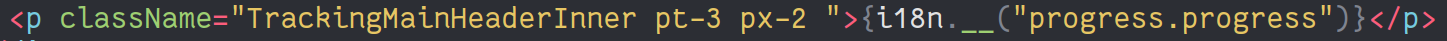
\includegraphics[width = 15cm]{src/public/oppar/translationcall.png}\\
Kuva \getImgCount. {} i18n käännösfunktiokutsu (ehkä uusi kuva)
\medskip

kuvassa luodaan HTML paragraafi elementti jossa kutsutaan käännösfunktiota. funktio hakee käännöstiedoston progress sivulta progress arvon.
\bigskip

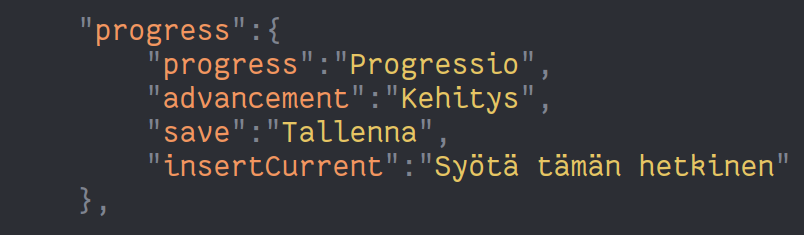
\includegraphics[width = 15cm]{src/public/oppar/translationfile.png}\\
Kuva \getImgCount. {} progressiosivun käännökset suomenkieliseltä käännöstiedostosta
\medskip

kuvassa progressio sivun käännökset. käännös tiedoston on json formaatissa joten sivut ovat omia objekteja. 
niiden ominaisuudet ovat avaimia mitä käytetään kun haetaan käännöksiä ja arvot ovat julkinen teksi.
Kuvassa \nextImageCount {} On Sama kohta käännöstiedostosta mutta englannin kielisestä.
\bigskip


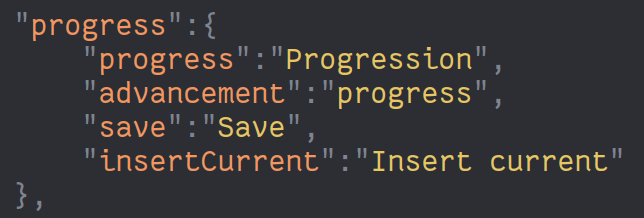
\includegraphics[width = 15cm]{src/public/oppar/translationfileEng.png}\\
Kuva \getImgCount {}. progressiosivun käännökset englanninkielisestä käännöstiedostosta(ehkä uusi kuva)
\medskip




% tämän kappaleen voisi poistaa. 
% lisätä tää toiseen kappaleeseen tai sitten poistaa kokonaan
\subsection{käyttöliittymä kielenvaihamiselle}

%lisäsin sivulle, tosin kun sivulle on lisätty
Sivulle on myös lisätty laskuvalikko kielen vaihtamiselle. 
Kielet kuvataan lippuina laskuvalikossa.
Liput toimivat nopeina visuaalisina vihjeinä, jotka auttavat käyttäjiä tunnistamaan haluamansa kielen.
kuvassa \nextImageCount.



\bigskip

\includegraphics[]{src/public/locale_laskuvalikko.png}\\
Kuva \getImgCount {}. Kielen vaihto laskuvalikko


\subsection{wip title kaksi}
Sovelluksen kaikki julkisesti oleva teksi on siirretty käännös tiedostoihin. 
Tämä luo keskitetyn sijainnin josta voi helposti etsiä ja korjata kirjoitus virheitä ja lisäämään uusia lauseita ja sanoja.
uuden kielen lisääminen vaatii uuden käännöstiedoston luomisen ja käännös arvojen asettelun tiedostoon.
\medskip

% saadaanko jotain lisää kirjoitettua ns "yhteenvetoon"










\newpage
\addPage{src/op/feature.tex}{Uuden ominaisuuden lisäys} % ------------------------------- FEATURE ------------------------------- %










\newpage
\section{Yhteenveto}             % ------------------------------- YHTEENVETO ------------------------------- %

sehän meni ihan hyvin 

opin käyttämään projektissa käytettyjä teknologioita
opin tekemään töitä ammatillisessa työympäristössä
\medskip


lokalisaatio meni hyvin ja sovellus on nyt parempi
\medskip


uusi ominaisuus toimii ja siitä ei tullut ognemlia sen käyttöönotossa
\medskip





\newpage

% we need some way to manually override an item when it looks like shit

% i thin we need to make our own @ thing then use that for htings that look like shit
% though i dont thik we need the hfill thing in the first place but whattever that is problem for another day


(korjaa outo spacing)
\bibliographystyle{labCitations} % ------------------------------- LÄHTEET ------------------------------- %
\bibliography{./src/op/citations}


%https://libguides.eur.nl/overleaf/bibliographies-and-citing
%https://tex.stackexchange.com/questions/51434/biblatex-citation-order
% i want to do citations like this but if there is problem with the format then must do manually or... write own system





\section{Liitteet}               % ------------------------------- Liitteet ------------------------------- %

miten laitan liitteen päiväkirjasta ja millainen se pitäisi olla








\end{document}
